



\vspace{-2mm}



%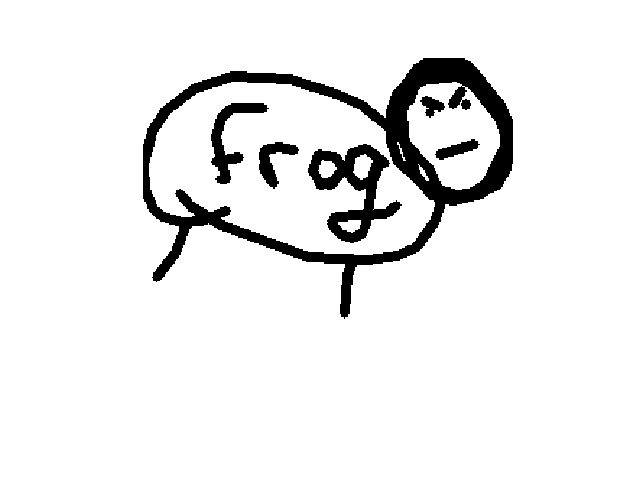
\includegraphics[width=0.5\textwidth]{figures/frog_draw_2.png}
%test texte

\begin{center}
Transformation de vecteurs de position en photos
\end{center}

\begin{center}

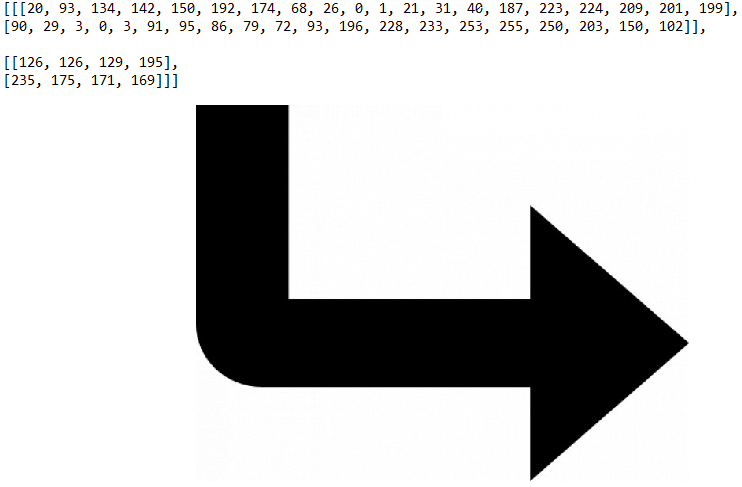
\includegraphics[width=15cm,height=15cm,keepaspectratio]{figures/vecteur_fleche.png}
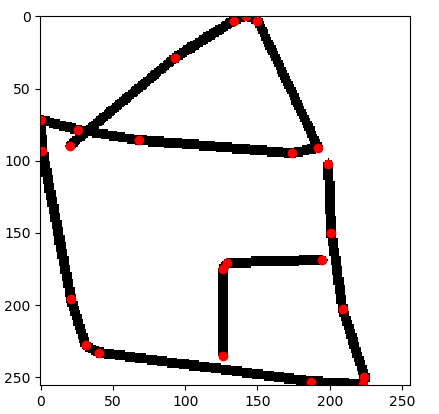
\includegraphics[width=15cm,height=15cm,keepaspectratio]{figures/housedraw.png}
%\captionof{figure}{Transformation des vecteurs }
\end{center}



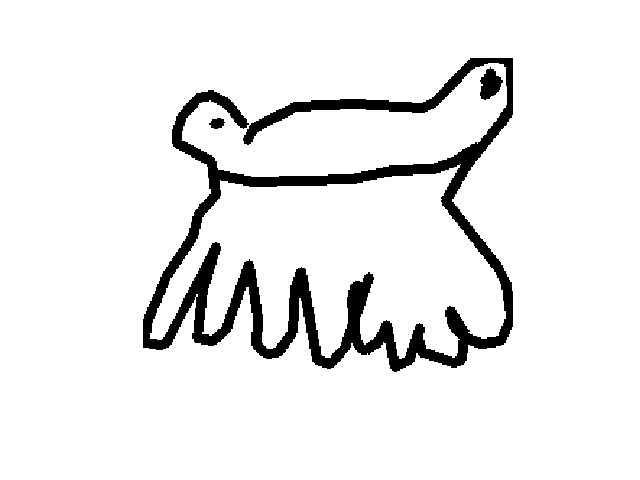
\includegraphics[width=10cm,height=10cm,keepaspectratio]{figures/frog_draw_1.png}
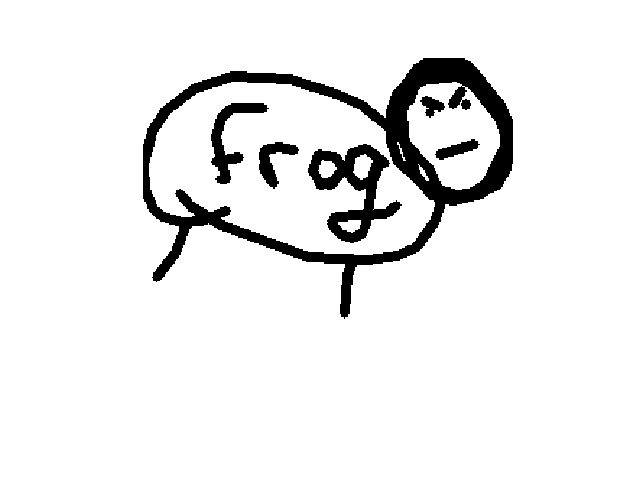
\includegraphics[width=10cm,height=10cm,keepaspectratio]{figures/frog_draw_2.png} \begin{itemize}
\item item 1
\item item 2!
\end{itemize}
%\captionof{figure}{Figure caption 1 (left); Figure caption 2 (right)}



\begin{multicols}{4}
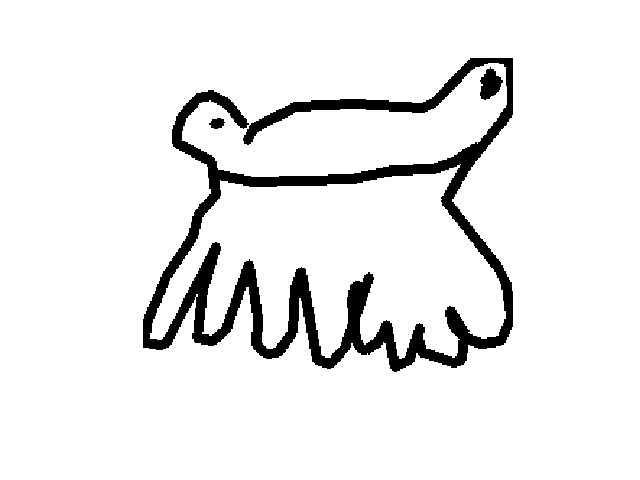
\includegraphics[width=10cm,height=10cm,keepaspectratio]{figures/frog_draw_1.png}
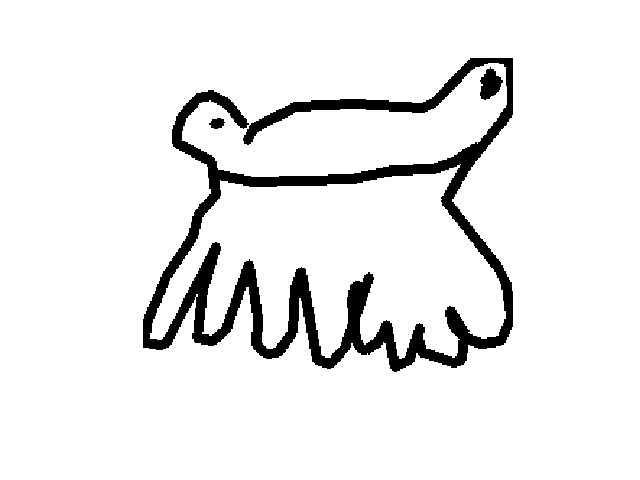
\includegraphics[width=10cm,height=10cm,keepaspectratio]{figures/frog_draw_1.png}
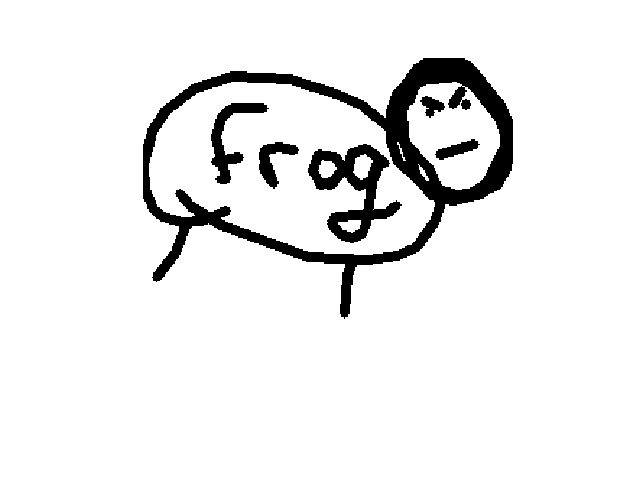
\includegraphics[width=10cm,height=10cm,keepaspectratio]{figures/frog_draw_2.png}

\begin{itemize}
\item item 1
\item item 2!
\end{itemize}
\end{multicols}





\begin{minipage}{0.3\textwidth}% adapt widths of minipages to your needs
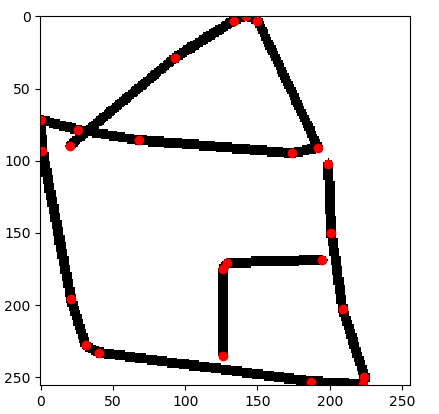
\includegraphics[width=10cm,height=10cm,keepaspectratio]{figures/housedraw.png}
\end{minipage}%

\begin{minipage}{0.6\textwidth}
Yesterday,\\
all my troubles seemed so far away\\
Now it looks as though they're here to stay\\
Oh, I believe in yesterday.
\end{minipage}






















\vspace{2mm}
Qualitative example on several OOV words (underlined). We can see that depending on the context and the target, the weights may shift drastically.
